\documentclass[12pt]{article}

% Author's up-front packages
\usepackage[T1]{fontenc}
\usepackage[utf8]{inputenc}

% Packages on template
\usepackage{amsmath, mathtools}
\usepackage{amsfonts}
\usepackage{amssymb}
\usepackage{graphicx}
\usepackage{colortbl}
\usepackage{xr}
\usepackage{hyperref}
\usepackage{longtable}
\usepackage{xfrac}
\usepackage{tabularx}
\usepackage{float}
\usepackage{siunitx}
\usepackage{booktabs}
\usepackage{caption}
\usepackage{pdflscape}
\usepackage{afterpage}

% ---- Author's choice to remove them ----
%\usepackage[round]{natbib}
%\usepackage{refcheck}

% Author's packages
\usepackage{cite}
\usepackage{indentfirst}
\usepackage{cleveref}
\usepackage{float}
%\usepackage{amsthm}
\usepackage{xcolor}
\definecolor{shadecolorIM}{RGB}{200,200,200}
\definecolor{shadecolorT}{RGB}{200,200,200}
\definecolor{shadecolorGD}{RGB}{200,200,200}
\definecolor{shadecolorDD}{RGB}{200,200,200}

\hypersetup{
    %bookmarks=true,			% show bookmarks bar?
    colorlinks=true,			% false: boxed links; true: colored links
    linkcolor=red,				% color of internal links (change box color with 
%linkbordercolor)
    citecolor=green,        % color of links to bibliography
    filecolor=magenta,      % color of file links
    urlcolor=blue           % color of external links
}

%% Comments

\usepackage{color}

\newif\ifcomments\commentstrue

\ifcomments
\newcommand{\authornote}[3]{\textcolor{#1}{[#3 ---#2]}}
\newcommand{\todo}[1]{\textcolor{red}{[TODO: #1]}}
\else
\newcommand{\authornote}[3]{}
\newcommand{\todo}[1]{}
\fi

\newcommand{\wss}[1]{\authornote{blue}{SS}{#1}}
\newcommand{\an}[1]{\authornote{magenta}{Author}{#1}}


% For easy change of table widths
\newcommand{\colZwidth}{1.0\textwidth}
\newcommand{\colAwidth}{0.13\textwidth}
\newcommand{\colBwidth}{0.82\textwidth}
\newcommand{\colCwidth}{0.1\textwidth}
\newcommand{\colDwidth}{0.05\textwidth}
\newcommand{\colEwidth}{0.8\textwidth}
\newcommand{\colFwidth}{0.17\textwidth}
\newcommand{\colGwidth}{0.5\textwidth}
\newcommand{\colHwidth}{0.28\textwidth}


% Used so that cross-references have a meaningful prefix
\newcommand{\progname}{STEM Moir{\'e} GPA}

\usepackage{fullpage}

%Set the custom referencing system
	% Goal Statement
\newtheorem{GS}{GS}
\crefname{GS}{GS}{GSs}
	% Assumption
\newtheorem{A}{A}
\crefname{A}{A}{As}
	% Theoretical Model
\newtheorem{T}{T}
\crefname{T}{T}{Ts}
	% Data Definition
\newtheorem{DD}{DD}
\crefname{DD}{DD}{DDs}
	% Data Constraints
\newtheorem{DC}{DC}
\crefname{DC}{DC}{DCs}
	% Instance Model
\newtheorem{IM}{IM}
\crefname{IM}{IM}{IMs}
	% General Definition
\newtheorem{GD}{GD}
\crefname{GD}{GD}{GDs}
	% Requirement
\newtheorem{R}{R}
\crefname{R}{R}{Rs}

\begin{document}

\title{Software Requirements Specifications (SRS) \\
STEM Moir{\'e} GPA} 
\author{Alexandre Pofelski \\
		macid: pofelska \\
		github: slimpotatoes}
\date{\today}
	
\maketitle

\pagenumbering{roman}
\tableofcontents

\begin{table}[bp]
\caption{\bf Revision History}
\begin{tabularx}{\textwidth}{p{3cm}p{2cm}X}
\toprule {\bf Date} & {\bf Version} & {\bf Notes}\\
\midrule
19/09/2017 & 1.0 & First Draft\\
\bottomrule
\end{tabularx}
\end{table}

\clearpage

\section{Reference Material}

\subsection{Table of Units}

Throughout this document SI 
(\href{<https://physics.nist.gov/cuu/Units/index.html>}{Syst\`{e}me 
Internationale d'Unit\'{e}s}) is employed as the unit system. In addition to the 
basic units, several derived units are used as described below.  For each unit, 
the symbol is given followed by a description of the unit and the SI name.\par 
\bigskip

\renewcommand{\arraystretch}{1.2}
%\begin{table}[ht]
  \noindent \begin{tabular}{l l l} 
    \toprule		
    \textbf{Symbol} & \textbf{Base quantity} & \textbf{Name SI}\\
    \midrule 
    \si{\metre} & length & metre\\
    \si{\per\metre} & reciprocal meter & wave number\\
    \si{\second} & time & second\\
    \bottomrule
  \end{tabular}
  %	\caption{Provide a caption}
%\end{table}

\wss{Only include the units that your SRS actually uses}

\subsection{Table of Symbols}

The table that follows summarizes the symbols used in this document along with
their units if applicable.

\renewcommand{\arraystretch}{1.2}
%\noindent \begin{tabularx}{1.0\textwidth}{l l X}
\noindent \begin{longtable*}{l l p{12cm}} \toprule
\textbf{Symbol} & \textbf{Unit} & \textbf{Description}\\
\midrule 
$\delta$ & & Dirac delta function \\
$\varepsilon$ & & Strain tensor \\
$\mathcal{FT}$ & & Fourier transform \\
$\overrightarrow{g_{hkl}}$ & \si{\per\nano\meter} & [hkl] crystalline wave vector \\
$i$ & & Imaginary unit \\
$\mathbb{N}$ & & Set of natural numbers\\
$\omega$ & & Rotation tensor\\
$p$ & \si{\nano\meter} & pixel size\\
$\mathbb{R}$ & & Set of real numbers\\
$\mathbb{Z}$ & & Set of integer numbers\\
\bottomrule
\end{longtable*}

\subsection{Abbreviations and Acronyms}

\renewcommand{\arraystretch}{1.2}
\begin{tabular}{l l} 
  \toprule		
  \textbf{symbol} & \textbf{description}\\
  \midrule 
  A & Assumption\\
  AU & Arbitrary Unit\\
  DC & Data Constraint \\
  DD & Data Definition\\
  EM & Electron Micrograph \\
  GD & General Definition\\
  GPA & Geometrical Phase Analysis \\
  GS & Goal Statement\\
  I & Intensity (or number of counts \\
  IM & Instance Model\\
  LC & Likely Change\\
  PS & Physical System Description\\
  R & Requirement\\
  SMH & STEM Moir{\'e} Hologram \\
  SRS & Software Requirements Specification\\
  STEM & Scanning Transmission Electron Microscopy \\
  T & Theoretical Model\\
  \bottomrule
\end{tabular}\\

\wss{Add any other abbreviations or acronyms that you add}

\newpage
\pagenumbering{arabic}

\section{Introduction}

\wss{This SRS template is based on \citet{SmithAndLai2005, SmithEtAl2007}.  It
  will get you started, but you will have to make changes.  Any changes to
  section headings should be approved by the instructor, since that implies a
  deviation from the template.  Although the bits shown below do not include
  type information, you may need to add this information for your problem.}


\wss{If you are documenting a family of models, you can start from this same
  template, but you will have to add a section for variabilities.  For program
  families you should look at \cite{Smith2006, SmithMcCutchanAndCarette2017}.
  You should be able to do one document that captures the commonality analysis
  and the requirements.}

\subsection{Purpose of Document}

\subsection{Scope of Requirements} 

\subsection{Characteristics of Intended Reader} 

\subsection{Organization of Document}

\section{General System Description}

This section identifies the interfaces between the system and its environment,
describes the user characteristics and lists the system constraints.

\subsection{System Context}

\wss{Your system context will likely include an explicit list of user and system
  responsibilities}

\begin{itemize}
\item User Responsibilities:
\begin{itemize}
\item 
\end{itemize}
\item \progname{} Responsibilities:
\begin{itemize}
\item Detect data type mismatch, such as a string of characters instead of a
  floating point number
\item 
\end{itemize}
\end{itemize}

\subsection{User Characteristics} \label{SecUserCharacteristics}

The end user of \progname{} should have an understanding of undergraduate Level
1 Calculus and Physics.

\subsection{System Constraints}

\wss{You may not have any system constraints}

\section{Specific System Description}
\subsection{Problem Description} \label{Sec_pd}

STEM Moir{\'e} GPA project is software capable of converting a STEM Moir{\'e} 
hologram into 2D strain maps.

\subsubsection{Terminology and Definitions}

Regarding the complexity of the electron/matter interaction, some crude 
simplifications are proposed to describe the terminologies below. While 
sometimes not realistic, the simplifications are here to help in visualizing the 
context and the type of data the STEM Moir{\'e} GPA software is subjected to. Nevertheless, 
all the simplifications are not affecting the definition of the concept used at 
the software level.

\begin{itemize}

\item \textbf{2D Cartesian coordinate system}: orthonormal coordinate system model by the orthonormal base $\mathcal{B}=(O,\vec{u_x},\vec{u_y})$ such that any vector $\vec{r}$ can be expressed as the following:
\begin{equation}
\forall (x,y) \in \mathbb{R}^{2}, \vec{r}=x\vec{u_x}+y\vec{u_y}
\end{equation}
\item \textbf{Pixel}: smallest addressable element sampling a 2D continuum.
\item \textbf{Electron Micrograph (EM)}: 2D array collected in an electron microscope 
representing the number of electron crossing the sample (intensity) at each 
pixel location.
\item \textbf{Scanning grid}: set representing the succession of the STEM probe positions when collecting the STEM EM. Equivalently the scanning grid represents the relative position of the pixel with respect to the sample when acquiring the EM. A simplified version of the 
STEM EM formation can be visualized in \cref{fig:STEM_imaging_Fig}. The positions of the STEM probe are located at the intersection of the black grid lines.
\begin{figure}[H]
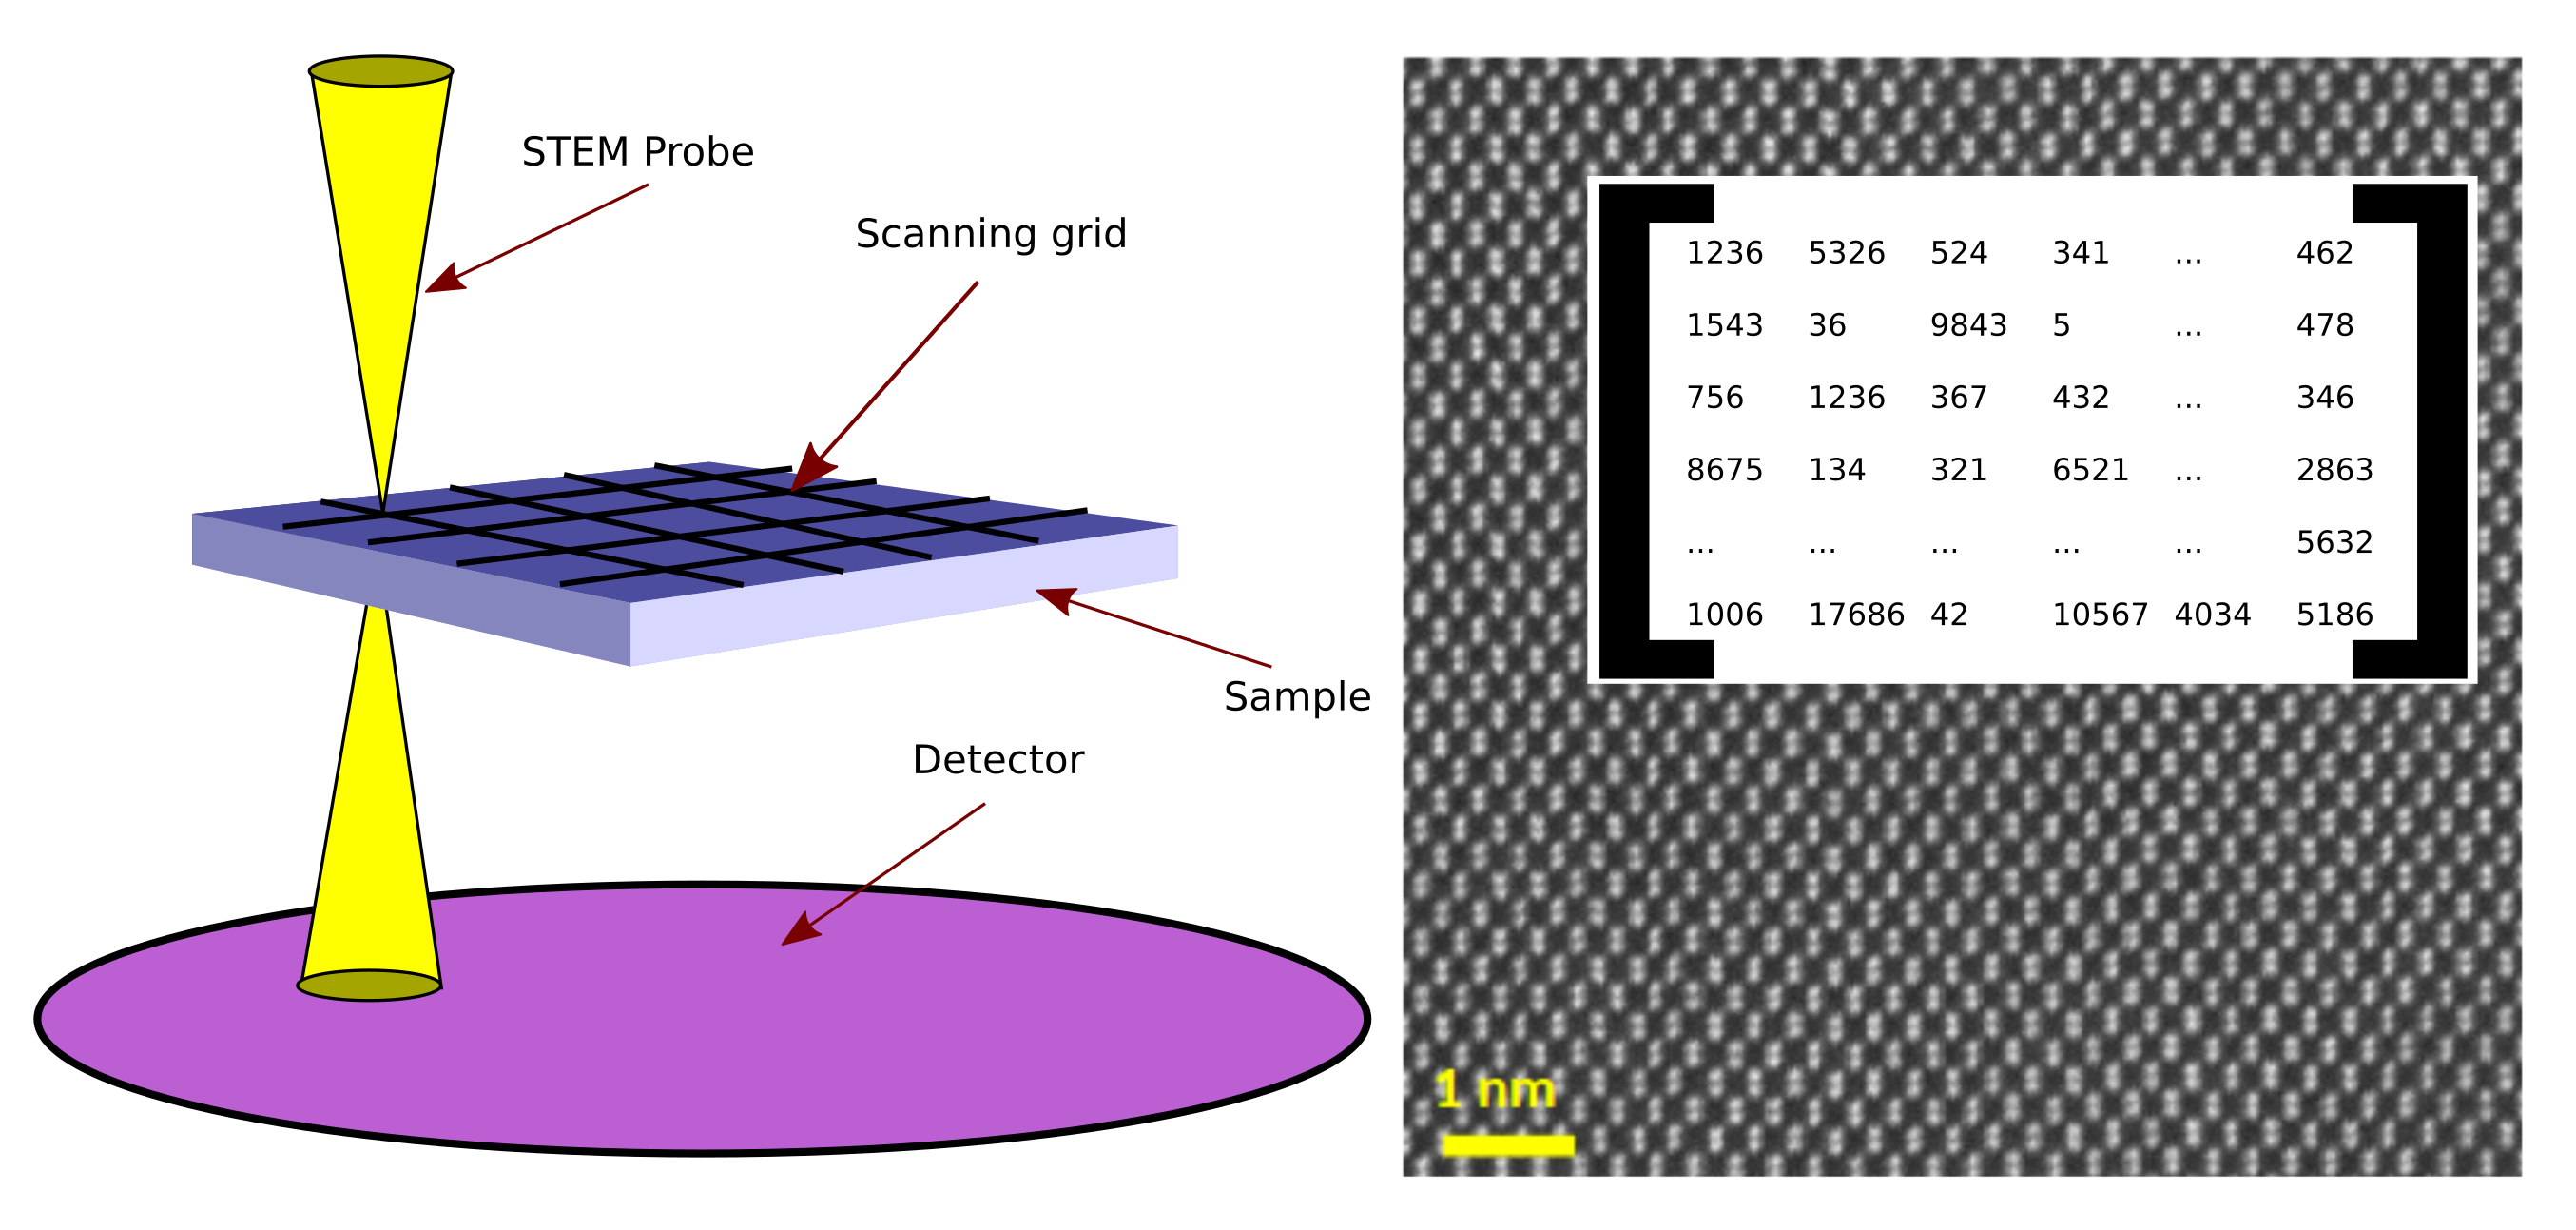
\includegraphics[width=\linewidth]{Figures/STEM_imaging_Fig.png}
\caption{On the left hand side, a schematic of the STEM EM formation with the STEM probe scanning the sample at each intersection of the grid lines. The electrons crossing the sample are collected on the detector and counted during the acquisition time. On the right hand side is presented a STEM EM on a pure silicon sample revealing its atomic structure. In the inset is highlighted the type of data the STEM EM corresponds to which is a 2D array.}
\label{fig:STEM_imaging_Fig}
\end{figure}
\item \textbf{Hologram}: Result from an interference between two or multiples waves. 
\item \textbf{Moir{\'e} hologram}: Result from interference between two or multiple waves with similar but not equal wave numbers (or wave vectors in 2D).
\item \textbf{Crystal lattice}: Arrangement of atoms forming matter.
\item \textbf{STEM Moir{\'e} hologram (SMH)}: EM collected in STEM and resulting from the 
Moir{\'e} interference between the scanning grid and the crystal lattice. 
\item \textbf{Strain map}: 2D array mapping the evolution of one element of the 2D strain or rotation 
tensor. 
\end{itemize}

\subsubsection{Physical System Description}

The physical system of \progname{}, as shown in Figure~?,
includes the following elements:


\wss{A figure here may make sense for most SRS documents}

% \begin{figure}[h!]
% \begin{center}
% %\rotatebox{-90}
% {
%  \includegraphics[width=0.5\textwidth]{<FigureName>}
% }
% \caption{\label{<Label>} <Caption>}
% \end{center}
% \end{figure}


\subsubsection{Goal Statements}

\noindent Given the system description, the goal statements are:
\begin{GS}
\normalfont Extract quantitatively the chosen crystalline wave vectors. This corresponds to extract $\vec{g_{j}}$ from $I_{SMH}$.
\label{GS_1}
\end{GS}
\begin{GS}
\normalfont Extract quantitatively the variation of the chosen crystalline wave vectors. This corresponds to extract $P_{g_{j}}$ from $I_{SMH}$.
\label{GS_2}
\end{GS}
\begin{GS}
\normalfont Display, on each pixel, all the elements of the 2D strain and rotation tensor which are the parameters $\varepsilon_{xx}$, $\varepsilon_{xy}$, $\varepsilon_{yy}$ and $\omega_{xy}$ in \cref{eq:strain_2}
\label{GS_3}
\end{GS}

\subsection{Solution Characteristics Specification}


\subsubsection{Assumptions}

\begin{A}
\normalfont The microscope has a limit of resolution corresponding to the probe size and thus cannot resolve any spatial frequency higher than $g_{j_{lim}}$. 
\label{A_1}
\end{A}
\begin{A}
\normalfont Since the STEM EM is discretized in pixels, the smallest features possible is composed of two pixels. Therefore, in reciprocal space, the maximum range of spatial frequency detectable is $\Gamma=[-\frac{1}{2p},\frac{1}{2p}]^{2}$.
\label{A_2}
\end{A}
\begin{A}
\normalfont The probe size is smaller than the area covered by one pixel. Therefore, information gathered on one pixel is only provided by the area covered by the pixel (no blurring).
\label{A_3}
\end{A}
\begin{A}
\normalfont The variation of the strain field (or deformation field) is small.
\label{A_4}
\end{A}
\begin{A}
\normalfont The strain magnitude is small (elastic regime).
\end{A}
\begin{A}
\normalfont The user knows the crystal structure of the sample analysed at its unstrained state or can provide a reference in which is embedded the crystal structure information at its unstrained state.
\label{A_6}
\end{A}

\subsubsection{Theoretical Models}\label{sec_theoretical}

\begin{T}
\normalfont \textbf{Sampling}
\begin{itemize}
\item \underline{Equation}: \Cref{eq:sampling_simplified}
\item \underline{Description}: In the 2D Cartesian coordinate system, the scanning grid can be seen as sampler $S$ of continuous function $f$. For the purpose of the STEM Moir{\'e} GPA, the sampler is set to be periodic with the same periodicity $p$ (called pixel size) in both $x$ and $y$ directions (2D Dirac comb). The resulting sampled version $f_S$ of $f$ can be represented as the following with $\delta$ representing the Dirac function:
\begin{equation}
\begin{gathered}
\forall (x,y) \in \mathbb{R}^{2}, f_S(x,y)=S(x,y)\times f(x,y) \\
\forall (x,y) \in \mathbb{R}^{2}, f_S(x,y)=\sum_{n=-\infty}^{n=+\infty}\sum_{m=-\infty}^{m=+\infty}\delta(x-np,y-mp)\times f(x,y)
\end{gathered}
\label{eq:sampling}
\end{equation}
For shorter notations, it is position to define a set Q as follows $Q=\{\forall (n,m) \in \mathbb{Z}^{2}, \vec{q}=n\vec{u_x}+m\vec{u_y}\}$ and thus simplify \cref{eq:sampling}
\begin{equation}
\forall (x,y) \in \mathbb{R}^{2}, f_S(\vec{r})=\sum_{q\in Q}\delta(\vec{r}-p\vec{q}) f(\vec{r})
\label{eq:sampling_simplified}
\end{equation}
\item \underline{Source}: Trouver un truc pr sampling (bouquin sur la table d'isobel
\item \underline{Ref by}:
\end{itemize}
\label{T_1}
\end{T}

\begin{T}
\normalfont \textbf{Geometrical Phase Analysis}
\begin{itemize}
\item \underline{Equation}: \Cref{eq:GPA_method}
\item \underline{Description}: Let consider a function $f$ decomposed in Fourier series as the following with 
\begin{equation}
\begin{gathered}
\forall \vec{r}=(x_1,...,x_n) \in \mathbb{R}^n, f(\vec{r})=\sum_{j=-\infty}^{j=+\infty}C_je^{i(\vec{k_j}\cdot\vec{r})} \\
\forall \vec{r}=(x_1,...,x_n) \in \mathbb{R}^n, f(\vec{r})=\sum_{j=-\infty}^{j=+\infty}A_je^{i((\vec{k_j}\cdot\vec{r})+B_j)}
\end{gathered}
\end{equation}
If there is a small perturbation locally of the n-dimensions wave vector $\vec{k_j}$, it is possible to model it allowing $B_j$ to be a function of $\vec{r}.$ 
\begin{equation}
\forall \vec{r}=(x_1,...,x_n) \in \mathbb{R}^n, f(\vec{r})=\sum_{j=-\infty}^{j=+\infty}A_je^{i((\vec{k_j}\cdot\vec{r})+B_j(\vec{r}))}
\end{equation}
The objective of GPA is to extract the perturbation, one chosen $B_j(\vec{r})$, from $f$ in Fourier space. Let's consider the Fourier transform of $f$ such that
\begin{equation*}
\begin{gathered}
\forall \vec{\nu}=(\nu_1,...,\nu_n) \in \mathbb{R}^n, \forall \vec{r}=(x_1,...,x_n) \in \mathbb{R}^n, \widetilde{f}(\vec{\nu})=\mathcal{FT}(f(\vec{r})) \\
\forall \vec{\nu}=(\nu_1,...,\nu_n) \in \mathbb{R}^n, \forall \vec{r}=(x_1,...,x_n) \in \mathbb{R}^n, \widetilde{f}(\vec{\nu})=\sum_{j=-\infty}^{j=+\infty}\mathcal{FT}(C_j(\vec{r})\times e^{i(\vec{k_j}\cdot\vec{r})})
\end{gathered}
\end{equation*}
\begin{equation}
\begin{gathered}
\forall \vec{\nu}\in \mathbb{R}^n, \widetilde{f}(\vec{\nu})=\sum_{j=-\infty}^{j=+\infty}\widetilde{C_j}(\vec{\nu})\ast\delta(\vec{\nu}-\vec{k_j})\\
\forall \vec{\nu}\in \mathbb{R}^n, \widetilde{f}(\vec{\nu})=\sum_{j=-\infty}^{j=+\infty}\widetilde{C_j}(\vec{\nu}-\vec{k_j})
\end{gathered}
\end{equation}
If all the $\vec{k_j}$ are separated enough to be isolated with a mask, then $B_j(\vec{r})$ can be extracted by considering the inverse Fourier transform of the masked area and expressing the result in term of amplitude and phase. In mathematical formalism, $B_j(\vec{r})$ is extracted as follows.
\begin{equation*}
\begin{gathered}
\text{if} \ \exists \ M :
\begin{array}{|ccl}
\mathbb{R}^{n} & \longrightarrow & \mathbb{C} \\
\vec{\nu} & \longmapsto & M(\vec{\nu}) 
    \end{array} / \begin{cases}
    					M(\vec{\nu}-\vec{k_j})\widetilde{f}(\vec{\nu})=\widetilde{C_j}(\vec{\nu}-\vec{k_j}) & \text{for} \ \vec{\nu} \in [(\nu_1^D,...,\nu_n^D),(\nu_1^U,...,\nu_n^U)] \\
    					M(\vec{\nu}-\vec{k_j})\widetilde{f}(\vec{\nu})=0 & 
    				 \end{cases} \\
\end{gathered}
\end{equation*}
\begin{equation}
\Rightarrow \begin{array}{l}
|\mathcal{FT}^{-1}[M(\vec{\nu})\widetilde{f}(\vec{\nu}+\vec{k_j})]|=|\mathcal{FT}^{-1}[\widetilde{C}(\vec{\nu})]|=A_j \\
arg(\mathcal{FT}^{-1}[M(\vec{\nu})\widetilde{f}(\vec{\nu}+\vec{k_j})])=arg(\mathcal{FT}^{-1}[\widetilde{C}(\vec{\nu})])=B_j(\vec{r})
\end{array}
\label{eq:GPA_method}
\end{equation}

\item \underline{Source}: \cite{Hytch1998,Rouviere2005}
\item \underline{Ref by}:
\end{itemize}
\label{T_2}
\end{T}

\subsubsection*{Description of the GPA method in a 1D coordinate system}
\noindent Let's consider a function $f$ such that 
\begin{equation*}
\begin{gathered}
\forall x \in \mathbb{R}, f(x)=C_0e^{i(k_0x)}+C_1e^{i(k_1x)} \\
\end{gathered}
\end{equation*}
Let's consider a small perturbation of $k_1$ modelled as the following
\begin{equation*}
\begin{gathered}
\forall x \in \mathbb{R}, f(x)=C_0e^{i(k_0x)}+A_1e^{i(k_1x)+iB_1(x)} \\
\end{gathered}
\end{equation*}
Applying the GPA method on $f$,
\begin{equation*}
\begin{gathered}
\forall \nu \in \mathbb{R}, \widetilde{f}(\nu)=C_0\delta(\nu-k_0)+\widetilde{C_1}(\nu)\ast\delta(\nu-k_1) \\
\forall \nu \in \mathbb{R}, \widetilde{f}(\nu)=C_0\delta(\nu-k_0)+\widetilde{C_1}(\nu-k_1)
\end{gathered}
\end{equation*}
Considering the perturbation around $k_1$ to be small and that $k_0$ and $k_1$ are enough separated such that the perturbation is located around $k_1$ in frequency space, it is possible to define a mask $M$ such that:
\begin{equation*}
\begin{gathered}
\forall \nu \in \mathbb{R}, M(\nu) = 
\begin{cases}
1 & \text{for} \ \nu-k_1 \in  [-\epsilon,+\epsilon] \ / \ k_0 \notin [k_1-\epsilon,k_1+\epsilon] \\
0
\end{cases}
\end{gathered}
\end{equation*}
In such case, multiply the mask $M$ with the Fourier transform of $f$ isolates $\widetilde{C_1}$ from the sum and can be independently transformed as follows:
\begin{equation*}
\begin{gathered}
\forall \nu \in \mathbb{R}, M(\nu-k_1)\widetilde{f}(\nu)=\widetilde{C_1}(\nu-k_1)
\end{gathered}
\end{equation*}
Setting, $\lambda=\nu-k_1$ and performing the inverse Fourier transform of the masked Fourier transform of $f$, the perturbation can be extracted.
\begin{equation*}
\begin{gathered}
\forall \nu \in \mathbb{R}, M(\lambda)\widetilde{f}(\lambda+k_1)=\widetilde{C_1}(\lambda) \\
\forall x \in \mathbb{R}, \mathcal{FT}^{-1}[M(\lambda)\widetilde{f}(\lambda+k_1)]=C_1(x) \\
\Rightarrow \begin{cases}
|C_1(x)|=A_1 \\
arg(C_1(x))=B_1(x)
\end{cases}
\end{gathered}
\end{equation*}
\begin{T}
\normalfont \textbf{Strain Model}
\begin{itemize}
\item \underline{Equation}: \Cref{eq:strain_2}
\item \underline{Description}: In infinitesimal strain theory with small displacement and small gradient of displacement, the displacement gradient tensor $\nabla u$ can be decomposed in two independent tensors: the symmetric strain tensor $\varepsilon$ and the anti-symmetric rotation tensor $\omega$. Their relationship can be described as follows:
\begin{equation}
\begin{gathered}
\nabla u = \varepsilon + \omega = \begin{bmatrix}
	\varepsilon_{xx} & \varepsilon_{xy} \\
	\varepsilon_{xy} & \varepsilon_{yy} 
	\end{bmatrix} + \begin{bmatrix}
	0 & \omega_{xy} \\
	-\omega_{xy} & 0 
	\end{bmatrix} \\ 
\varepsilon = \frac{1}{2}(\nabla u+(\nabla u)^{T}) \\
\omega = \frac{1}{2}(\nabla u-(\nabla u)^{T})
\end{gathered}
\label{eq:strain_2}
\end{equation}
\item \underline{Source}:\cite{Hytch1998,Rouviere2005}
\item \underline{Ref by}:
\end{itemize}
\label{T_3}
\end{T}

\begin{T}
\normalfont \textbf{Interferometry}
\begin{itemize}
\item \underline{Equation}: \Cref{eq:hologram}
\item \underline{Description}: Let consider two monochromatic plane waves $\psi_1$ and $\psi_2$ with their respective amplitude $A_j$, phase $\phi_j$ and wave vector $\vec{k_j}$ in the 2D Cartesian system interfering with each other. The resulting hologram $\psi_H$ represented by the intensity $I_H$ can be modelled as follows with :
\begin{equation}
\forall (x,y) \in \mathbb{R}^{2}, \psi_H(\vec{r})=\psi_1+\psi_2= A_1e^{i(\vec{k_1}\cdot\vec{r})+i\phi_1}+A_2e^{i(\vec{k_2}\cdot\vec{r})+i\phi_2}
\end{equation}
\begin{equation}
\begin{split}
\forall (x,y) \in \mathbb{R}^{2}, I_H(\vec{r})=\psi_H\psi_H^{*}= & A_{1}^{2}+A_{2}^{2}+ \\ & A_{1}A_{2}(e^{i(\vec{k_1}-\vec{k_2})\cdot\vec{r}+i(\phi_1-\phi_2)}+e^{i(\vec{k_2}-\vec{k_1})\cdot\vec{r}+i(\phi_2-\phi_1)})
\end{split}
\label{eq:hologram}
\end{equation}
The more waves are contributing to the hologram, the more complex \cref{eq:hologram} will be. However, similar factors will appear with constants and cross product terms.
\item \underline{Source}:
\item \underline{Ref by}:
\end{itemize}
\label{T_4}
\end{T}

\subsubsection{General Definitions}\label{sec_gendef}

\begin{GD}
\normalfont \textbf{Strain in crystal lattice}
\begin{itemize}
\item \underline{Equation}: \Cref{eq:Strain_GPA}
\item \underline{Description}: For the purpose of the STEM Moir{\'e} GPA, only mono-crystalline samples are analysed. In the case of a perfect periodic atomic arrangement, the crystalline lattice $I_c$ can be described in Fourier series with $C_j$ the complex Fourier coefficient related to the crystalline wave vector $\vec{g_j}$ in the 2D Cartesian system.
\begin{equation}
\forall (x,y) \in \mathbb{R}^{2},I_C(\vec{r})=\sum_{j=-\infty}^{j=+\infty}C_je^{i(\vec{g_j}\cdot\vec{r})}
\label{eq:crystal_Fourier_series}
\end{equation}
If the crystal is elastically deformed, the relative position of the atoms will be slightly modified from their original unstrained configuration. The local deformation is breaking locally the perfect periodicity of the crystalline lattice. In the case of small deformation, $C_j$ can be allowed to vary in space in \cref{eq:crystal_Fourier_series}. Representing $C_j$ with a phase $A_j$ and an amplitude $P_j$, a pure displacement is only contributing in the phase component. The strain information is therefore embedded in $P_{g_{j}}(\vec{r})$ such that $P_{g_{j}}(\vec{r})=2\pi\Delta \overrightarrow{g_{j}}(\vec{r})\cdot\vec{r}$ where $\Delta \overrightarrow{g_j}$ represent the variation of the crystalline vector compared to its unstrained state.
\begin{equation}
\begin{gathered}
\forall (x,y) \in \mathbb{R}^{2},I_C(\vec{r})=\sum_{j=-\infty}^{j=+\infty}C_j(\vec{r})e^{i(\vec{g_j}\cdot\vec{r})} \\
\forall (x,y) \in \mathbb{R}^{2},I_C(\vec{r})=\sum_{j=-\infty}^{j=+\infty}A_je^{i(\vec{g_j}\cdot\vec{r})+iP_{g_{j}}(\vec{r})}
\end{gathered}
\label{eq:crystal_strain_Fourier_series}
\end{equation}
By applying GPA (\cref{T_2}) on \cref{eq:crystal_strain_Fourier_series}, $P_{g_{j}}(\vec{r})$ can be extracted. Then by applying \cref{A_4}, the gradient $\nabla$ of $P_{g_{j}}(\vec{r})$ can be approximate as follows
\begin{equation}
\nabla P_{g_{j}}(\vec{r}) = 2\pi [\nabla( \Delta \overrightarrow{g_j}(\vec{r}))]^T\vec{r}  + 2\pi\Delta \overrightarrow{g_j(\vec{r})} \approx 2\pi\Delta \overrightarrow{g_j(\vec{r})}
\label{eq:Strain_GPA}
\end{equation}
\item \underline{Source}: \cite{Hytch1998}
\item \underline{Ref by}:
\end{itemize}
\label{GD_1}
\end{GD}

\begin{GD}
\normalfont \textbf{STEM Moir{\'e} hologram}
\begin{itemize}
\item \underline{Equation}: \Cref{eq:SMH_simplified_1}
\item \underline{Description}: Combining \cref{eq:crystal_strain_Fourier_series} and \cref{eq:sampling}, a STEM Moir{\'e} hologram $I_{SMH}$ can be described as follows
\begin{equation}
\forall (x,y) \in \mathbb{R}^{2}, I_{SMH}(\vec{r})=\sum_{q\in Q}\delta(\vec{r}-p\vec{q})\times\sum_{j=-\infty}^{j=+\infty}A_je^{i(\vec{g_j}\cdot\vec{r})+iP_{g_{j}}(\vec{r})}
\label{eq:SMH_1}
\end{equation}
By modifying $p$ the scanning periodicity (or the pixel size), it is possible to adjust the spatial frequency of the SMH solving \cref{eq:SMH_1}.Applying \cref{A_1}, the expression of $I_C$ in \cref{eq:crystal_strain_Fourier_series} is simplified since the series becomes a finite sum.
\begin{equation}
\forall (x,y) \in \mathbb{R}^{2},I_C(\vec{r})=\sum_{j=-j_{lim}}^{j=+j_{lim}}A_je^{i(\vec{g_j}\cdot\vec{r})+iP_{g_{j}}(\vec{r})}
\label{eq:crystal_lattice_simplified}
\end{equation}
Therefore, the STEM Moir{\'e} hologram $I_{SMH}$ is also simplified as follows:
\begin{equation}
\forall (x,y) \in \mathbb{R}^{2}, I_{SMH}(\vec{r})=\sum_{q\in Q}\delta(\vec{r}-p\vec{q})\times\sum_{j=-j_{lim}}^{j=+j_{lim}}A_je^{i(\vec{g_j}\cdot\vec{r})+iP_{g_{j}}(\vec{r})}
\label{eq:SMH_simplified_1}
\end{equation}
\item \underline{Source}:\cite{Pofelski2017}
\item \underline{Ref by}:
\end{itemize}
\label{GD_2}
\end{GD}

\subsubsection*{From sampling to a hologram}

Since the Dirac comb function is also periodic, the sampler can also be represented into Fourier series
\begin{equation}
\forall (x,y) \in \mathbb{R}^{2}, S(\vec{r})=\sum_{q\in Q}\delta(\vec{r}-p\vec{q}) = \frac{1}{(2\pi)^2}\sum_{q\in Q}\sum_{l=-\infty}^{l=+\infty}e^{il(\vec{r}-p\vec{q})}
\label{eq:SMH_2}
\end{equation}
Using \cref{eq:SMH_2} in \cref{eq:SMH_simplified_1}, it is possible to recognize an interference equation between multiple plane waves (a more complex version of \cref{eq:hologram}).
\begin{equation}
I_{SMH}(\vec{r})=\frac{1}{(2\pi)^2}\sum_{q\in Q}\sum_{l=-\infty}^{l=+\infty}\sum_{j=-j_{lim}}^{j=+j_{lim}}A_je^{i(\vec{g_j}\cdot\vec{r}+l(\vec{r}-p\vec{q}))+iP_{g_{j}}(\vec{r})}
\label{eq:SMH_3}
\end{equation}

\begin{GD}
\normalfont \textbf{Deformation gradient tensor}
\item \underline{Equation}: \Cref{eq:strain_1}
\item \underline{Description}: If $\vec{g_j}=g_{j_{x}}\vec{u_{x}}+g_{j_{y}}\vec{u_{y}}$ and $\Delta \vec{g_{j}}=\Delta g_{j_{x}}\vec{u_{x}}+\Delta g_{j_{y}}\vec{u_{y}}$ are known in the base $\mathcal{B}$ for two non-collinear crystalline wave vectors, then the strain deformation tensor can be deduced by calculating first both the unstrained matrix $G$ and the variation of the crystalline wave vectors matrix $\Delta G$. Then the deformation gradient tensor $\nabla u$ is estimated as the following with $I_{d}$ representing the identity matrix (see annexe D in ref{Hytch1998} and equation (30) in ref{Rouviere2005}). 
\begin{equation}
\begin{gathered}
	G_{ref} =
	\begin{bmatrix}
	g_{1_{x}} & g_{1_{y}} \\
	g_{2_{x}} & g_{2_{y}} 
	\end{bmatrix} \\
	\Delta G =
	\begin{bmatrix}
	\Delta g_{1_{x}} & \Delta g_{1_{y}} \\
	\Delta g_{2_{x}} & \Delta g_{2_{y}} 
	\end{bmatrix} \\
\nabla u = ({\Delta G}^{T})^{-1}{G_{ref}}^{T}-I_{d}
\end{gathered}
\label{eq:strain_1}
\end{equation}
\item \underline{Source}:\cite{Hytch1998,Rouviere2005}
\item \underline{Ref by}:
\label{GD_3}
\end{GD}

\subsubsection{Data Definitions}\label{sec_datadef}

\renewcommand{\labelitemi}{$\star$}

\begin{DD}
\normalfont \textbf{Experimental STEM Moir{\'e} hologram}
\begin{itemize}
\item {Symbol}: $I_{SMH_{exp}}$
\item {Unit}: Intensity (AU)
\item {Description}: 2D array
\item {Ref by}:
\end{itemize}
\label{DD_1}
\end{DD}

\begin{DD}
\normalfont \textbf{Fourier transform of the experimental STEM Moir{\'e} hologram}
\begin{itemize}
\item {Symbol}: $\widetilde{I}_{SMH_{exp}}$ 
\item {Unit}: Intensity (AU)
\item {Description}: 2D array
\item {Ref by}:
\end{itemize}
\label{DD_2}
\end{DD}

\begin{DD}
\normalfont \textbf{Reference crystal wave vector}
\begin{itemize}
\item {Symbol}: $\overrightarrow{g_{j}}^{C_{ref}}$ 
\item {Unit}: \si{\per\nano\metre}
\item {Description}: 2D vector
\item {Ref by}:
\end{itemize}
\label{DD_3}
\end{DD}

\begin{DD}
\normalfont \textbf{Reference crystal structure}
\begin{itemize}
\item {Symbol}: $I_{C_{ref}}$
\item {Unit}: Intensity (AU)
\item {Description}: 2D array
\item {Ref by}:
\end{itemize}
\label{DD_4}
\end{DD}

\begin{DD}
\normalfont \textbf{Simulated SMH from reference crystal structure and scanning grid}
\begin{itemize}
\item {Symbol}: $I_{SMH_{sim}}$
\item {Unit}: Intensity (AU)
\item {Description}: 2D array
\item {Ref by}:
\end{itemize}
\label{DD_5}
\end{DD}

\begin{DD}
\normalfont \textbf{Fourier transform of the $I_{SMH_{sim}}$}
\begin{itemize}
\item {Symbol}: $\widetilde{I}_{SMH_{sim}}$
\item {Unit}: Intensity (AU)
\item {Description}: 2D array
\item {Ref by}:
\end{itemize}
\label{DD_6}
\end{DD}

\begin{DD}
\normalfont \textbf{Experimental Moir{\'e} wave vector}
\begin{itemize}
\item {Symbol}: $\overrightarrow{g_{j}}^{M_{exp}}$
\item {Unit}: \si{\per\nano\metre}
\item {Description}: 2D vector
\item {Ref by}:
\end{itemize}
\label{DD_7}
\end{DD}

\begin{DD}
\normalfont \textbf{Sampling vector operating in $\Gamma$ frequency range}
\begin{itemize}
\item {Symbol}: $\overrightarrow{q_{j}}$
\item {Unit}: \si{\per\nano\metre}
\item {Description}: 2D vector
\item {Ref by}:
\end{itemize}
\label{DD_8}
\end{DD}

\begin{DD}
\normalfont \textbf{Mask isolating a spatial frequency}
\begin{itemize}
\item {Symbol}: $M$
\item {Unit}: Intensity (AU)
\item {Description}: 2D array
\item {Ref by}:
\end{itemize}
\label{DD_9}
\end{DD}

\begin{DD}
\normalfont \textbf{Masked Fourier transform of experimental STEM Moir{\'e} hologram}
\begin{itemize}
\item {Symbol}: $M\widetilde{I}_{SMH_{exp}}$
\item {Unit}: Intensity (AU)
\item {Description}: 2D array
\item {Ref by}:
\end{itemize}
\label{DD_10}
\end{DD}

\begin{DD}
\normalfont \textbf{Experimental Crystalline wave vector}
\begin{itemize}
\item {Symbol}: $\overrightarrow{g_{j}}^{C_{exp}}$
\item {Unit}: \si{\per\nano\metre}
\item {Description}: 2D vector
\item {Ref by}:
\end{itemize}
\label{DD_11}
\end{DD}

\begin{DD}
\normalfont \textbf{Geometric phase image}
\begin{itemize}
\item {Symbol}: $P_{\Delta\overrightarrow{g_{j}}^{M_{exp}}}$
\item {Unit}: rad
\item {Description}: 2D array
\item {Ref by}:
\end{itemize}
\label{DD_12}
\end{DD}

\begin{DD}
\normalfont \textbf{Unstrained area in the geometric phase image}
\begin{itemize}
\item {Symbol}: $U$
\item {Unit}: Dimensionless
\item {Description}: 2D array
\item {Ref by}:
\end{itemize}
\label{DD_13}
\end{DD}

\subsubsection{Instance Models} \label{sec_instance}    

\renewcommand{\labelitemi}{$-$}

\begin{IM}
\noindent\colorbox{shadecolorIM}{\normalfont \textbf{Simulate the SMH on a reference to determine $\overrightarrow{q_{j}}$ for each $\vec{g_j}^{M}$}}
\normalfont
\begin{itemize}
\item Input: $I_{C_{ref}}, p$
\item Output: $I_{SMH_{sim}}, \overrightarrow{q_{j}}, \overrightarrow{g_j}^{M_{ref}}$
\item Source:
\item Ref by:
\end{itemize}
\label{IM_1}
\end{IM}

\begin{IM}
\noindent\colorbox{shadecolorIM}{\normalfont \textbf{GPA on a selected Moir{\'e} wave vector from $I_{SMH_{exp}}$}}
\normalfont
\begin{itemize}
\item Input: $I_{SMH_{exp}}, M$
\item Output: $P_{\Delta \overrightarrow{g_{j}}^{M_{exp}}}$
\item Source:
\item Ref by:
\end{itemize}
\label{IM_2}
\end{IM}

\begin{IM}
\noindent\colorbox{shadecolorIM}{\normalfont \textbf{Determine an unstrained area in the geometric phase image}}
\normalfont
\begin{itemize}
\item Input: $P_{\Delta \overrightarrow{g_{j}}^{M_{exp}}},U$
\item Output: $\overrightarrow{g_{j}}^{M_{exp}}$
\item Source:
\item Ref by:
\end{itemize}
\label{IM_3}
\end{IM}

\begin{IM}
\noindent\colorbox{shadecolorIM}{\normalfont \textbf{Convert the Moir{\'e} wave vector into the Crystalline wave vector}}
\normalfont
\begin{itemize}
\item Input: $\overrightarrow{g_{j}}^{M_{exp}},\Delta \overrightarrow{g_{j}}^{M_{exp}},\overrightarrow{q_{j}},p$
\item Output: $\Delta \overrightarrow{g_{j}}^{C_{exp}},\overrightarrow{g_{j}}^{C_{exp}}$
\item Source:
\item Ref by:
\end{itemize}
\label{IM_4}
\end{IM}

\begin{IM}
\noindent\colorbox{shadecolorIM}{\normalfont \textbf{Strain calculation using 2 non-crystalline wave vectors}}
\normalfont
\begin{itemize}
\item Input: $g_{1_{x}}^{C_{exp}}, g_{1_{y}}^{C_{exp}},g_{2_{x}}^{C_{exp}}, g_{2_{y}}^{C_{exp}}, \Delta g_{1_{x}}^{C_{exp}}, \Delta g_{1_{y}}^{C_{exp}},\Delta g_{2_{x}}^{C_{exp}},\Delta g_{2_{y}}^{C_{exp}}$
\item Output: $\varepsilon_{xx},\varepsilon_{xy},\varepsilon_{yy},\omega_{xy}$
\item Source:
\item Ref by:
\end{itemize}
\label{IM_5}
\end{IM}

\subsubsection{Data Constraints} \label{sec_DataConstraints}    

\subsubsection{Properties of a Correct Solution} \label{sec_CorrectSolution}

\noindent
A correct solution must exhibit \wss{fill in the details}

\section{Requirements}

This section provides the functional requirements, the business tasks that the
software is expected to complete, and the nonfunctional requirements, the
qualities that the software is expected to exhibit.

\subsection{Functional Requirements}



\subsection{Nonfunctional Requirements}

\wss{List your nonfunctional requirements.  You may consider using a fit
  criterion to make them verifiable.}

\section{Likely Changes}    


\section{Traceability Matrices and Graphs}


\wss{You will have to modify these tables for your problem.}

\newpage

\bibliography{SRS_biblio}
\bibliographystyle{ieeetr}


\newpage

\section{Appendix}

\wss{Your report may require an appendix.  For instance, this is a good point to
show the values of the symbolic parameters introduced in the report.}

\subsection{Symbolic Parameters}



\end{document}
